% Standalone teaser: a population of items is produced on the left, split by a
% property, and routed to two consumers on the right; an inset shows what the
% downstream operation does to the vectors it receives.
%
% Contains no measured results. Every coordinate below is drawn, not fitted; the
% inset geometry is stated exactly in the comments so a reader can reproduce it.
%
% Build:
%   mkdir -p /tmp/teaser-build
%   pdflatex -interaction=nonstopmode -halt-on-error \
%            -output-directory=/tmp/teaser-build 10_teaser_flow.tex
%   cp /tmp/teaser-build/10_teaser_flow.pdf figures/teaser.pdf
%   pdftoppm -scale-to 2100 -png -singlefile figures/teaser.pdf figures/teaser
%
% Place at 1:1 with \includegraphics[width=\linewidth]{figures/teaser}.
\documentclass[tikz,border=3pt]{standalone}
\usepackage{newtxtext,newtxmath}   % Times body, matching a times template
\usepackage{amsmath}
\usetikzlibrary{arrows.meta,calc}

% Google brand colours at the medium tier, the same sheet figures/style.py uses;
% ink, soft, and faint are that sheet's neutrals.
\definecolor{ink}{HTML}{333333}
\definecolor{soft}{HTML}{5F6368}
\definecolor{faint}{HTML}{CCCCCC}
\definecolor{hueA}{HTML}{6FA1F2}   % ordinary items
\definecolor{hueB}{HTML}{F2C33F}   % the item the figure is about
\definecolor{hueC}{HTML}{DE6F66}   % the method

\tikzset{
  every node/.style={font=\fontsize{10}{12}\selectfont,text=ink,inner sep=0pt},
  flow/.style={-{Stealth[length=2mm,width=1.5mm]},draw=soft,line width=.85pt},
  vector/.style={-{Stealth[length=2mm,width=1.5mm]},line width=1.1pt},
  ghost/.style={-{Stealth[length=1.8mm,width=1.3mm]},line width=.8pt,
                densely dashed,opacity=.32},
  note/.style={font=\fontsize{9}{11}\selectfont,text=soft,align=center},
  label/.style={font=\fontsize{10.5}{12}\selectfont},
  box/.style={draw=faint,fill=white,rounded corners=3pt,minimum width=1.55cm,
              minimum height=.67cm,font=\fontsize{12}{14}\selectfont},
}

% One row of the item population: #1,#2 = origin, #3 = last index, #4 = colour.
\newcommand{\itemrow}[4]{%
  \foreach \i in {0,...,#3}{%
    \fill[#4!42,rounded corners=.5pt] (#1+\i*.18,#2) rectangle ++(.125,.12);}%
}

\begin{document}
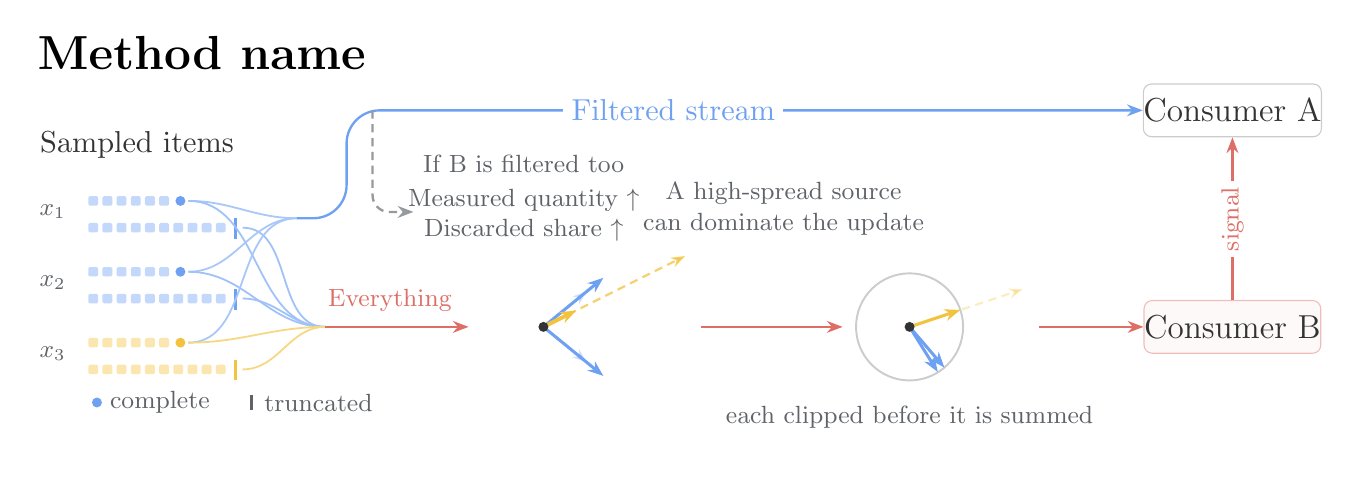
\begin{tikzpicture}[x=1cm,y=-1cm]           % y down, so the figure reads top to bottom
\path[use as bounding box] (0,0) rectangle (16.4,5.6);
\node[anchor=west,font=\fontsize{16}{18}\selectfont\bfseries,text=black]
      at (.12,.32) {Method name};

% Two consumers on the right. The upper one sees a filtered stream, the lower
% one sees everything, and the lower one feeds the upper.
\node[box] (up) at (15.3,1.05) {Consumer A};
\node[box,draw=hueC!45,fill=hueC!4] (down) at (15.3,3.80) {Consumer B};
\draw[flow,hueC] (down.north) -- (up.south);
\node[note,rotate=90,text=hueC,fill=white,inner sep=2pt] at (15.3,2.43) {signal};

% The population: three rows, each a group of items under one source.
\node[label,anchor=west] at (.15,1.49) {Sampled items};
\foreach \yy/\col/\lab in {2.14/hueA/1, 3.04/hueA/2, 3.94/hueB/3}{
  \node[note,anchor=east] at (.49,\yy+.20) {$x_{\lab}$};
  \itemrow{.77}{\yy}{5}{\col}
  \fill[\col] (1.94,\yy+.06) circle (1.8pt);           % terminal marker: complete
  \itemrow{.77}{\yy+.34}{9}{\col}
  \draw[\col,line width=1pt] (2.64,\yy+.28) -- (2.64,\yy+.54);  % cut bar: truncated
  \draw[hueA!60,line width=.65pt] (2.04,\yy+.06) to[out=0,in=180] (3.42,2.42);
  \draw[\col!65,line width=.65pt] (2.04,\yy+.06) to[out=0,in=180] (3.78,3.80);
  \draw[\col!65,line width=.65pt] (2.73,\yy+.40) to[out=0,in=180] (3.78,3.80);
}
% The key is two marks, not two colours: colour is already carrying the source.
\fill[hueA] (.88,4.76) circle (1.8pt);
\node[note,anchor=west] at (1.04,4.76) {complete};
\draw[soft,line width=1pt] (2.84,4.66) -- (2.84,4.86);
\node[note,anchor=west] at (3.00,4.76) {truncated};

\draw[flow,hueA,rounded corners=12pt] (3.42,2.42)--(4.05,2.42)--(4.05,1.05)--(up.west);
\node[label,fill=white,inner sep=3pt,text=hueA] at (8.2,1.05) {Filtered stream};
% The lower path is one pipeline: everything -> weighting -> clipping -> B.
\draw[flow,hueC] (3.78,3.80) -- (5.60,3.80);
\node[note,text=hueC,fill=white,inner sep=2pt] at (4.60,3.46) {Everything};
\draw[flow,hueC] (8.55,3.80) -- (10.35,3.80);
\draw[flow,hueC] (12.85,3.80) -- (down.west);

% The consequence of filtering both consumers, drawn as a dashed branch.
\draw[flow,soft!65,densely dashed,rounded corners=6pt]
      (4.38,1.05)--(4.38,2.34)--(4.90,2.34);
\node[note] at (6.30,1.73) {If B is filtered too};
\node[note] at (6.30,2.38) {Measured quantity $\uparrow$\\Discarded share $\uparrow$};

% Inset: inverse-spread weighting rescales each vector without rotating it.
% Vectors (.55,.45), (.55,-.45), (1.8,-.9); spreads 1:1:6; normalized weights
% 18/13, 18/13, 3/13. Solid = weighted, dashed = original.
\coordinate (W) at (6.55,3.80);
\draw[ghost,hueA] (W) -- ++(.55,-.45);
\draw[ghost,hueA] (W) -- ++(.55,.45);
\draw[ghost,hueB,opacity=.75] (W) -- ++(1.8,-.9);
\draw[vector,hueA] (W) -- ++(.76154,-.62308);
\draw[vector,hueA] (W) -- ++(.76154,.62308);
\draw[vector,hueB,line width=1.4pt] (W) -- ++(.41538,-.20769);
\fill[ink] (W) circle (1.8pt);
\node[note] at (9.6,2.30) {A high-spread source\\can dominate the update};

% Second inset: each contribution is clipped inside one norm circle before they
% are summed. Threshold 1, display scale .68 cm per unit; the dashed extension
% identifies the outlier before clipping.
\coordinate (K) at (11.2,3.80);
\draw[faint,line width=.7pt] (K) circle (.68);
\draw[ghost,hueB] (K) -- ++(1.44,-.48);
\draw[vector,hueA] (K) -- ++(.3577,.5724);
\draw[vector,hueA] (K) -- ++(.4426,.5164);
\draw[vector,hueB] (K) -- ++(.6452,-.2151);
\fill[ink] (K) circle (1.8pt);
\node[note] at (11.2,4.95) {each clipped before it is summed};

\end{tikzpicture}
\end{document}
